\chapter{Literature Review}
\section{Drone Dynamics and Control}
\subsection{Drone Dynamics}
Mathematical models form the basis of any description of a dynamic system. There are large bodies of literature dedicated to modelling a quadrotors dynamics, to various complexities. The dynamic model seeks to describe the 3D position of the quadrotor. In aircraft terms, this is usually described with measurements such as altitude, and longitude / latitude coordinates. This may also be accompanied with a heading - the direction the aircraft is facing relative to a compass. Other measurements exist to define the position and direction of a drone within a 3D space. The dynamic model is a set of mathematical equations comprising of the sum of forces acting on the system at a time $t$. The various models can be divided into two main categories: models that do not incorporate the motor (body models) and models that do incorporate the motor (propulsion system modelling). The latter type may also incorporate the propellers into the model \cite{hd1}.

DiCesare \textit{et al} present a Lagrangian model for a quadrotor, utilising the `thrust of each motor' as a control input \cite{hd2}. Waslander \textit{et al} utilise a Newton-Euler method to derive a body model, also giving an approximate relationship between motor torque and voltage applied to the motors \cite{hd3}. Acakpovi \textit{et al} use a quaternion representation to achieve body modelling, seeking to achieve a more comprehensive and adaptable body model \cite{hd4}. Das \textit{et al} address the complexities and unknowns of certain elements of the mathematical model by using a backstepping approach and neural nets on their Lagrangian body model to estimate aerodynamic forces and moments \cite{hd5}. All of these models utilise various assumptions such as, the body is rigid and centre of mass and structure are coincident and symmetrical. From these works, the fact that there are numerous approaches to body models, where different goals and capabilities can be seen. The different models underline the importance of both the physical components and the mathematical relationships in understanding and controlling drone behaviour for particular applications.

Propulsion system models can present themselves in various levels of complexity. The vast majority of physical drones and consequently, drone models within literature, use brushless DC motors.  Wierema presents the modelling case of a brushless DC motor in the context of drones \cite{hd6}. Bouabdallah \textit{et al} derive a linearised DC motor model to be used in conjunction with a Lagrangian body model \cite{hd7}. Köroğlu presents a neural network approach to model the motor \cite{hd8}. Propeller modelling also falls under the scope of increasing the granularity and accuracy of the drone model. %Huang \textit{et al} identify the various aerodynamic coefficients and equations of a propeller blade in the context of a drone \cite{hd-drone-modeling} CHECK. 
Ryll \textit{et al} combine a Newton-Euler body model with a propeller model to achieve full controllability over the degrees of freedom of a quadrotor \cite{hd9}. Pounds \textit{et al} robustly model propeller flapping within their mathematical model to achieve a more accurate model \cite{hd10}. Motor models and the integration of propeller models, as showcased in the literature, underscore the increasing sophistication and precision required in advancing drone control, with increasingly granular models seeking to solve specific issues. 
\subsection{Drone Control}
The field of automated control for flying vehicles has been the subject of significant scientific interest. Control techniques rely on simplifying models, with limited states and inputs. However, it is essential to consider what are the critical elements for these reduced models to ensure the reliability of the control guidelines when applied to real aircraft. The quadrotor is a highly sophisticated flying vehicle owing to its exceptional versatility and manoeuvrability, enabling it to carry out a diverse range of tasks \cite{li6}. 

Robust control systems have gained considerable attention in mitigating parameter uncertainties and external disturbances. Uncertainties arising from changes in propeller rotation, blade flapping, propeller rotation speed, and the position of the centre of mass require the use of a robust nonlinear controller, especially in the case of quadrotors. Maintaining control over all six degrees of freedom in quadrotors is challenging due to the limited number of control inputs relative to the number of degrees of freedom; in essence, quadrotors represent an under-actuated system \cite{EMRAN2018165}. To regulate the height, speed, and direction of drones, the altitude controller plays a crucial role in guiding the drone during take-off and landing phases, while control of the drone's direction and speed is vital for successful flight over designated way-points. Li \textit{et al} propose a propose an altitude controller that consists of a PD control term and an acceleration feedback term for a tail-sitter UAV \cite{li7}. 

To meet these control requirements, a variety of control systems can be employed, such as proportional-integral derivative (PID), linear quadratic regulator (LQR), sliding mode control (SMC), fuzzy logic, neural network (NN), and others \cite{li8}. PID controllers are commonly used in autopilot systems due to their simple implementation, but they have limitations in unexpected and hostile environments. Linear quadratic regulation (LQR) provides optimal control methods for managing dynamic systems by minimising an appropriate cost function. When LQR is combined with a linear quadratic estimator (LQE) and a Kalman filter, the result is known as a Linear Quadratic Gaussian (LQG) controller \cite{li9}. Sliding mode control is a nonlinear control technique that employs a discontinuous control signal to direct the system to ``slide'' along a predetermined trajectory. On the other hand, Model Predictive Control (MPC) is another nonlinear approach used to govern UAVs. MPC employs a dynamic model of the system to forecast future states and solve optimal control problems online while minimising error. 

Analysing the literature researched above, traditional methods such as PID, LQR, and sliding mode control offer certain advantages, they may exhibit limitations when faced with unpredictable or hostile environments. Thus, the exploration of more adaptive, nonlinear approaches such as MPC, fuzzy logic, and neural networks in literature seems promising, potentially leading to more effective control in terms of adaptability, error minimisation, and trajectory optimisation.
\begin{comment}
There are several challenges and limitations in controlling the pitch, yaw, and roll dynamics of quadrotor drones. These include: 

Nonlinear and Coupled Dynamics: The dynamic equations of motion for quadrotor drones are inherently nonlinear and coupled, making it difficult to design efficient and robust controllers \cite{Rehan17}. This nonlinearity stems from factors such as aerodynamic effects, motor and propeller dynamics, and the interaction between rotational and translational motions. Traditional linear control techniques may not provide adequate performance and stability in scenarios requiring stabilisation due to multi-angle disturbances, requiring the development of advanced nonlinear control strategies \cite{7016810,hd-cite3}.

External Disturbances: Drones are susceptible to disturbances such as wind, which can significantly impact their stability and control performance. Controllers must be capable of adapting to these disturbances to maintain the desired flight trajectory. Moreover, disturbances can vary rapidly in magnitude and direction, demanding robust and adaptive control algorithms that can adjust in real-time to maintain stability and performance \cite{Kangunde2021}.

Actuator Limitations: The motors and propellers used in quadrotor drones have limitations in terms of their maximum and minimum thrust levels, as well as their response times. These limitations can affect the drone's ability to achieve the desired pitch, yaw, and roll angles. Additionally, actuator saturation or failure can lead to a loss of control authority, making it challenging to maintain stability and perform desired manoeuvres \cite{Joshi2022}. 

Sensor Noise: The onboard sensors, such as inertial measurement units (IMUs) and GPS, are susceptible to noise and inaccuracies, which can impact the controller's ability to estimate the drone's state. These uncertainties can propagate through the control loop and degrade the overall performance and stability \cite{190940}. Advanced filtering techniques, such as the Extended Kalman Filter or the Particle Filter, are often employed to mitigate the effects of sensor noise and improve state estimation \cite{hd-kalman_filter}. 

Model Uncertainty: Accurate mathematical models of quadrotor dynamics are essential for control design. However, these models may not perfectly capture the real-world behaviour of the drone due to factors such as unmodelled aerodynamic effects, manufacturing imperfections, and changes in mass distribution due to payload or battery depletion \cite{hd-drone-modeling}. Model uncertainty can lead to a mismatch between the controller's assumptions and the actual drone dynamics, resulting in reduced performance and potential instability \cite{hd-uav_modelling}.  

Computational Constraints: Advanced control algorithms often require significant computational resources to solve complex optimization problems or implement adaptive techniques in real-time. The limited processing power and memory available on small drones can constrain the choice of control algorithms and their implementation, potentially impacting the overall control performance. Drones | Free Full-Text | Computationally-Efficient Distributed Algorithms of Navigation of Teams of Autonomous UAVs for 3D Coverage and Flocking (mdpi.com) Miniaturizing the brain of a drone | Robotics @ MIT 

Robustness and Fault Tolerance: Ensuring robustness and fault tolerance in quadrotor control systems is crucial for maintaining stability and preventing catastrophic failures in the event of component malfunction, such as motor or sensor failure Fault-Tolerant Control of an Hexarotor Unmanned Aerial Vehicle Applying Outdoor Tests and Experiments - ScienceDirect. Designing controllers that can automatically detect and adapt to such failures, or even enable the drone to perform a controlled emergency landing, remains a significant challenge Automated Emergency Landing System for Drones: SafeEYE Project | IEEE Conference Publication | IEEE Xplore viewcontent.cgi (usu.edu). 
\end{comment}
\subsection{Model Predictive Control}
Model Predictive Control (MPC) is a increasingly popular control method tested in several applications including autonomous vehicles and medical uses. The results from literature for MPC suggest that it is a robust and efficient control method, however can be inflexible and hard to implement in some cases. As there has been more extensive testing on MPC, this review looks to find literature that compares the use of ANFIS and MPC controllers. 

A research paper by Rodriguez \textit{et al} tested designs for a controller for exoskeletons, devices used augment patient rehabilitation, specifically in a re-configurable exoskeleton for lower limbs \cite{zain11}. In this paper, the performance of PD, ANFIS and MPC controllers were tested in this application and can be seen in Figure \ref{fig:mpc}. This shows that the MPC and ANFIS controllers have a lower average error in position than the PD controller. When comparing the MPC and ANFIS controller results, the MPC is better at certain points, however, the paper concludes that the ANFIS controller performs better for this application. This shows the flexibility and ease of implementation of ANFIS could result in it being favourable in complex applications.  
\begin{figure}[H]
    \centering
    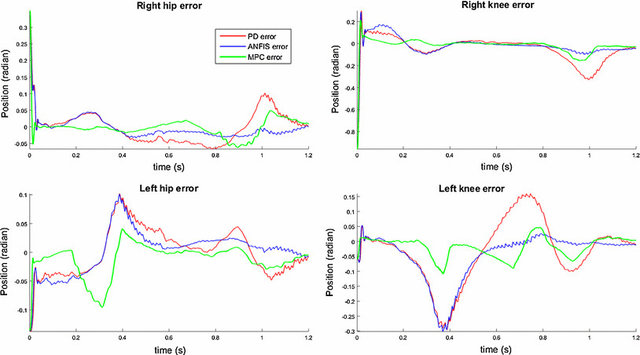
\includegraphics[width = 0.75\textwidth]{img/mpc_results.jpg}
    \caption[Research paper showing error in positions results for PD, ANFIS and MPC controllers]{Research paper showing error in positions results for PD, ANFIS and MPC controllers \cite{zain11}.} 
    \label{fig:mpc}
\end{figure} 
\subsection{Extended Kalman Filter}
The Kalman Filter is an efficient optimal estimator that provides an iterative computational methodology for estimating the state of a discrete-data controlled process from measurements that are usually noisy, whilst also giving an estimate of the uncertainty of the estimates \cite{zain12}. The Extended Kalman Filter (EKF) is an extension of this, where non-linearities are accounted for. This method can also be used as an alternative to the PID control method and has proven to be useful in literature. 

Few papers have been written directly comparing the use of EKF and learning-based methods for controllers as most papers compare the results of PID, MPC and learning-based approaches. This could suggest that EKFs are known to be less effective for controllers and therefore investigating this in recent years has not been worthwhile. A journal by Aydogmus \textit{et al} compared the use of Extended Kalman Filter and ANN approaches to estimate shaft speed for a closed-loop control system \cite{zain14}. This paper found that the Artificial Neural-Networks (ANN) implementation produced better performance than the EKF. Another research paper by Cuevas \textit{et al} directly compared an ANFIS model to an EKF model in the application of gaze control \cite{zain13}. Gaze control refers to using computational tricks to alter one's gaze. The results from the paper can be seen in Figure \ref{fig:kalman}. The results show that the EKF has a much higher number of frames at a higher error. These studies support the fact that EKF methods may generally be regarded as inferior in control applications when compared to learning-based approaches. 
\begin{figure}[H]
    \centering
    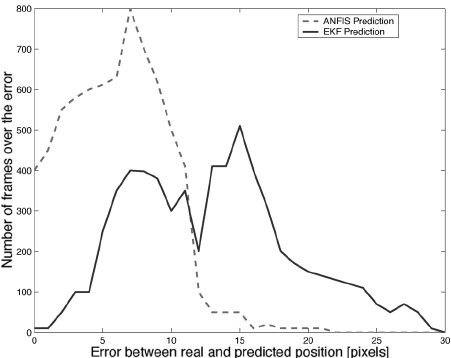
\includegraphics[width = 0.7\textwidth]{img/kalman filter.png}
    \caption[Performance results of EKF compared with ANFIS for gaze control]{Performance results of EKF compared with ANFIS for gaze control \cite{zain13}.}
    \label{fig:kalman}
\end{figure} 
\subsection{Neural Network Based Control}
Learning-based controllers use different variations of neural network approaches. As the framework of neural networks is inspired by the human brain and is a widely used machine learning method,  it follows that variations of this learning-based technique are used for controllers. 

A research paper by Arora \textit{et al} compared the use of ANN and ANFIS based controllers for grid connected photovoltaic (PV) systems. As PV arrays have non-linear characteristics, from changing temperature and solar irradiation, these learning-based algorithms are crucial for tracking maximum power from the PV array \cite{zain9}. The control response for both controllers were compared and the ANFIS controller had a lower settling time, overshoot, and fewer oscillations when compared with the ANN controller. Conclusively, in this application, an ANFIS controller performed better. 

Another research paper by Uluocak \textit{et al} analysed the use of different learning models applied to an Eddy Current Dynamometer \cite{zain10}. An Eddy Current Dynamometer is an instrument used to convert mechanical energy to electrical energy. This paper found that the ANFIS model performed better than the Radial Basis Neural Network (RBNN) and the Single Hidden Layer Neural Network (SHLNN) as it produced the lowest Mean Absolute Percentage Error (MAPE). As a result, it can be concluded from literature, that in complex control applications, ANFIS is likely to provide the most promising results. 
\section{Current Studies on Neuro-Fuzzy Controllers}
\subsection{Review on fuzzy-neural network controllers} 
Adaptive Neuro-Fuzzy Inference System (ANFIS) is a powerful hybrid method, which combines the advantages of fuzzy logic and neural networks to establish an efficient decision-making system \cite{boxi1}. Recently, ANFIS has significant applications in unmanned aerial vehicles (UAVs) such as path planning and obstacle avoidance. In this review, we will study the existing literature on ANFIS-based control systems compared with conventional proportional integral derivative (PID) controllers for the operation of UAVs and autonomous drones. 
%When ANFIS is used in the optimisation of the autonomous drones, the collected data from using a traditional PID controller act as inputs ($x$ and $y$) in Figure \ref{fig:anfis}. 

Figure \ref{fig:anfis} shows a generic ANFIS architecture, accepting inputs from a PID controller. In this instance $x$ and $y$ represent two generic inputs from data collected from a PID controller. In the fuzzification process seen in Layer 1, the computer reacts like a human brain and gives out linguistic outputs, such as ``low speed''. Layer 2, the product layer, then determines the rules that will be used to make decisions based on the fuzzy variables generated in Layer 1. At this stage, an optional normalisation layer can be implemented, however, if the inputs are already between 0 and 1, this can be excluded. Layer 4, the defuzzification layer, then converts the outputs from Layer 2 / 3 into a defuzzified output that feeds into the output layer \cite{boxi2}. 
\begin{figure}[H]
    \centering
    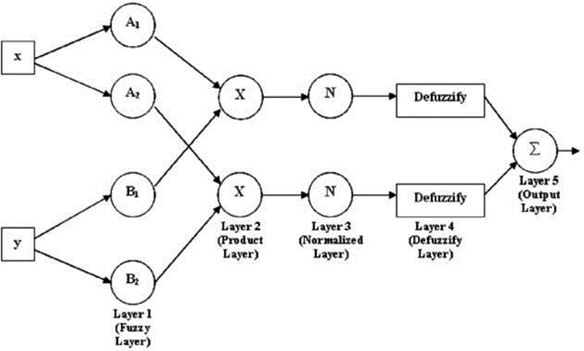
\includegraphics[width = 0.8 \textwidth]{img/Picture1.png}
    \caption[Architecture of an ANFIS model.]{Architecture of an ANFIS model \cite{boxi2}.}
    \label{fig:anfis}
\end{figure}
Recent studies on utilising ANFIS in control applications include an innovative approach for the autonomous flight control of UAVs using ANFIS. ANFIS mainly consists of three stages: input-output mapping, fuzzy inference, and rule optimisation, which can also be implemented into the quadrotors \cite{boxi4}. The input-output mapping stage involves collecting data on the flight performance (altitude, air speed and bank angle), which is then used to train the ANFIS model. The fuzzy inference stage uses the trained ANFIS model to make decisions on the  flight control based on its current and desired states. The rule optimisation stage aims to improve the performance of the ANFIS model by refining the fuzzy rules and adjusting the membership functions. Kurnaz \textit{et al} introduce three fuzzy logic modules to control the three-dimensional position of a UAV by adjusting the roll and pitch angles and throttle position \cite{boxi3}. This ANFIS model has 5 layers, with a hybrid learning algorithm based on a Sugeno inference system, which reduced the response time and made the controller more efficient. 

The authors tested their approach on a simulated UAV and evaluated its performance based on several metrics, including error in altitude, speed, and heading angle. The results in the paper show that the ANFIS-based approach outperforms a conventional PID controller in terms of design simplicity and trajectory following. However, unstable performance is caused by inconsistent ANFIS learning algorithms during the change of environmental conditions such as wind speed. The obstacle avoidance also has similar issues due to the change of positions of obstacles and the learning algorithm should be carefully monitored. This provides a framework and a set of results which can be built on. 

Another approach on quadrotors by Al-Fetyani \textit{et al} presents a novel ANFIS-based control system that integrates a fuzzy inference system (FIS) and a neural network (NN) to enhance the accuracy and robustness of the drone control system, particularly its attitude (direction relative to the horizon line) and altitude performances \cite{boxi5}. The article outlines the design and implementation of ANFIS, which involves three stages: data collection, model training, and controller development. Attitude and altitude data is collected from a flight simulation using a classical PD controller. The ANFIS-PD controller is trained and designed by a neuro-fuzzy designer. The training stage gives the membership functions for the inputs of altitude and attitude errors as well as their error rates. 

The design methodology involves building an ANFIS-based model to predict the output values of the drone's attitude and altitude control systems. The data acquisition and pre-processing steps involve collecting sensor data from the drone and filtering it to remove noise and outliers, which makes the data clearer and easier to process by ANFIS. Therefore, data cleaning after collection is a necessary step to ensure the ANFIS model can be trained optimally. The performance of controllers is evaluated using simulation experiments, where the quadrotor is subjected to various flight scenarios. 

Case 1 is taken from Luukkonen’s research on modelling and control of quadrotor \cite{boxi6}. The simulation results shown in Figure \ref{fig:referencepic} demonstrate that the ANFIS-PD controller can achieve the desired state in the shortest time with minimal overshooting. In addition, the power consumption of PD controller is more than twice as much as the ANFIS controller. As compared with a conventional PD controller, Fuzzy-PD still has a better performance.
\begin{figure}[H]
    \centering
    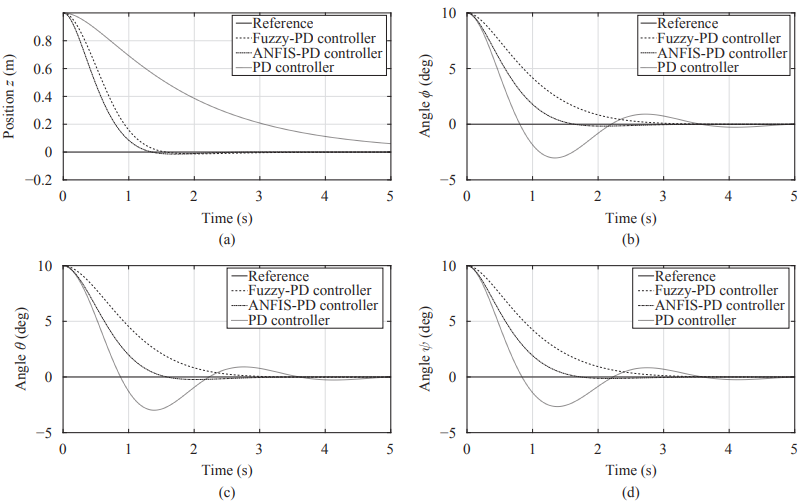
\includegraphics[width = 0.7 \textwidth]{img/Picture2.png}
    \caption[Simulation results for case 1: (a) Position z; (b) Angle $\phi$; (c) Angle $\theta$; (d) Angle $\varphi$.]{Simulation results for case 1: (a) Position z; (b) Angle $\phi$; (c) Angle $\theta$; (d) Angle $\varphi$ \cite{boxi5}.}
    \label{fig:referencepic}
\end{figure}
This analysis was then built on by Al-Fetyani to develop a case 2. In this case, the desired state varies over time. Since the PD controller is tuned to a near hovering state, within the time interval of 10-\SI{15}{\second}, oscillations occur while attempting to regulate the angular positions $\phi$ and $\varphi$. In comparison with PD and Fuzzy-PD controllers, the time required for ANFIS-PD controller to reach the desired state is still the fastest in this case. A case 3 was then developed, which looked into the performance of the controllers in following a desired altitude when subjected to disturbances. In this case of the ANFIS-PD controller, it has considerable resilience in the presence of external forces. The analysis performed on these cases also provide a basis for further analysis and once again shows the potential improvements applying ANFIS in a controller provides. 

The results show that the ANFIS can improve the attitude and altitude performances of the drone, which has low error rates with external disturbance force and fastest response times to reach a time varying state compared to conventional control methods. In the quadrotor, results of positions in $x$, $y$ and $z$ direction for different cases using fuzzy neural controller and PID controller are compared with the desired position. Another approach is on trajectory tracking of marine rescue drone by Pham and Han \cite{boxi7}. The main challenge in these operations is the ability to accurately track a desired trajectory and compensate for disturbances such as wind. The neural network estimates the drone's position and velocity based on sensor data, and the fuzzy logic controller generates control signals based on the estimated position and velocity. Simulations of PID and fuzzy neural controllers adjusting $z$ position of the drone are carried out in the conditions of presence and absence of wind. The graph of attitude varies with time from Figure \ref{fig:picture5} and Figure \ref{fig:picture6} demonstrates that the fuzzy neural controller is much more effective than a PID controller. 
\begin{figure}[H]
\centering
\begin{minipage}{.5\textwidth}
    \centering
    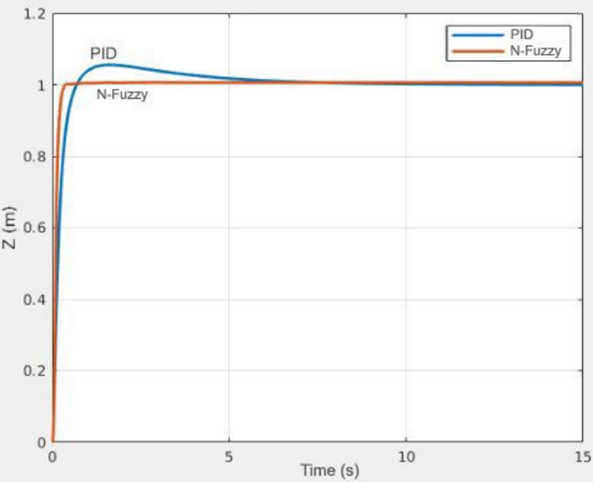
\includegraphics[width=0.95\linewidth]{img/Picture5.png}
    \caption[Simulation result of attitude against time for PID and N-Fuzzy controllers without wind.]{Simulation result of attitude against time for PID and N-Fuzzy controllers without wind \cite{boxi7}.}
    \label{fig:picture5}
\end{minipage}%
\begin{minipage}{.5\textwidth}
    \centering
    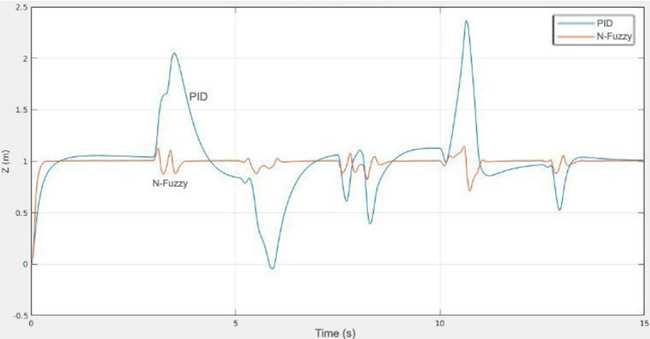
\includegraphics[width=0.95\linewidth]{img/Picture6.png}
    \caption[Simulation result of attitude against time for PID and N-Fuzzy controllers with wind.]{Simulation result of attitude against time for PID and N-Fuzzy controllers with wind \cite{boxi7}.}
    \label{fig:picture6}
\end{minipage}
\end{figure}
The graph of drone’s thrust over time using PID and neural fuzzy controller in Figure \ref{fig:picture7} and Figure \ref{fig:picture8} illustrates that the neural fuzzy controller has a shorter response time than the PID controller, with a more effective reaction on the action of wind. In the case of the drone's obstacle avoidance, the simulation result is also comparable to the performance of the two controllers with and without disturbance.

The performance of ANFIS was evaluated using simulations and experiments, and the results showed that the neuro-fuzzy controller was able to accurately track the desired trajectory and compensate for disturbances. It reaches a stable state faster with a larger thrust, which improves the efficiency by 67\% and reduced the response time by 85\% compared with PID controllers \cite{boxi7}. This study demonstrates the performance metrics used to evaluate both controllers and shows the use of error in $z$ position and error in thrust as the two chosen response curves.   
\begin{figure}[H]
\centering
\begin{minipage}{.5\textwidth}
    \centering
    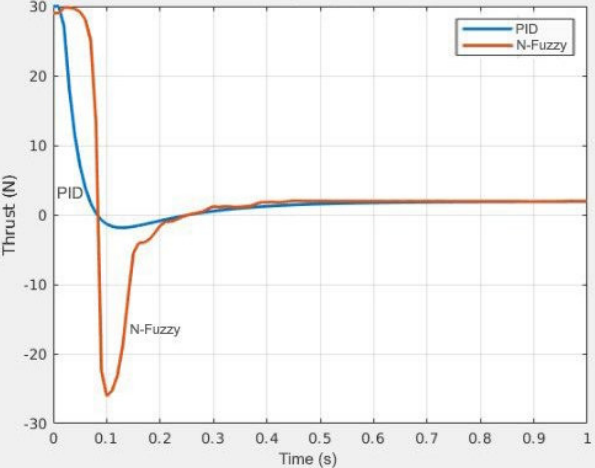
\includegraphics[width=0.95\linewidth]{img/Picture7.png}
    \caption[Simulation result of thrust against time for PID and N-Fuzzy controllers without wind.]{Simulation result of thrust against time for PID and N-Fuzzy controllers without wind \cite{boxi7}.}
    \label{fig:picture7}
\end{minipage}%
\begin{minipage}{.5\textwidth}
    \centering
    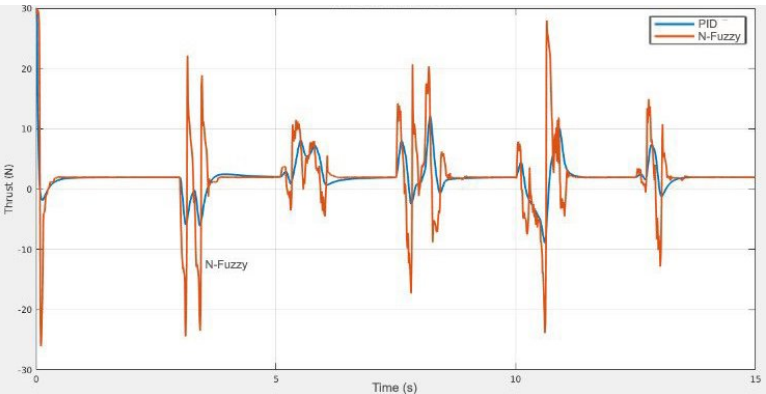
\includegraphics[width=0.95\linewidth]{img/Picture8.png}
    \caption[Simulation result of thrust against time for PID and N-Fuzzy controllers with wind.]{Simulation result of thrust against time for PID and N-Fuzzy controllers with wind \cite{boxi7}.}
    \label{fig:picture8}
\end{minipage}
\end{figure}
\subsection{Type-1 and Type-2 Fuzzy Inference Systems} 
Fuzzy Inference Systems (FIS) have been widely used in the development of autonomous drones for various applications. Type-1 and Type-2 FIS are inference systems where two different types of fuzzy sets are used to build the FIS. Type-1 FIS is based on crisp logic and is the most common FIS in autonomous drones \cite{boxi8}. However, more recent studies are analysing the use of Type-2 FIS and whether, in some applications, these types perform better.

Research on Type-2 fuzzy systems by Castañón-Puga \textit{et al} is an extension of Type-1 fuzzy systems that can handle uncertainties and non-linearity in the input data \cite{boxi9}. A self-learning Type-2 fuzzy system is presented, which is a system that can adapt and learn from data in real time. The Type-2 FIS was developed in order to build a mobile application that uses Wi-Fi signals to obtain indoor locations. Therefore, for this application, this study found that a Type-2 fuzzy system was more adequate. 

A case study of a self-learning Type-2 FIS by Al-Mahturi is applied to the control of an autonomous underwater vehicle \cite{boxi10}. The system uses data from the vehicle’s sensors and the result shows that Type-2 FIS can effectively identify the system’s dynamics and control the vehicle’s motion to follow a desired path, concluding that self-learning Type-2 fuzzy systems have great potential in system identification and control of autonomous systems. 

A study by Ontiveros \textit{et al} compared Type-1 and Type-2 systems in medical diagnosis \cite{zain3}. The conclusions of the study were that for data sets with low uncertainty, Type-1 fuzzy inference systems performed the best and that for data sets with medium and high uncertainty, Type-2 FIS performed the best. Therefore, despite the use of Type-2 systems in autonomous underwater vehicles and results from Al-Mahturi \textit{et al}, the best configuration of FIS for a drone application will highly depend on the data set used to train the FIS. 

\subsection{Sugeno versus Mamdani Fuzzy Inference Systems} 
Mamdani and Sugeno are two Fuzzy Inference Systems (FIS) developed by Takagi-Sugeno and Professor Ebrahim Mamdani. Mamdani FIS is characterised by its defuzzification output of membership function, whereas Sugeno FIS has a crisp output computed by a weighted average \cite{boxi11}. As a result, Sugeno FIS are generally better in applications of optimisation, pattern recognition and control systems whereas Mamdani FIS are better in applications of education, training, consumer-orientated applications and highly complex applications. Both have been used in various applications of drone technology, including trajectory tracking, obstacle avoidance, and aerial surveillance.

In trajectory tracking, Mamdani FIS has been used to control the movement of drones. For example, in the study by Pham and Han, a combined neural network and Mamdani FIS was used to control the trajectory of a marine rescue drone \cite{boxi7}. The Mamdani FIS was used to determine the velocity and heading of the drone based on the input variables, which included the current location of the drone, the location of the target, and the obstacle avoidance status. It provides a smooth and stable control of the drone trajectory. 

In aerial surveillance, both Mamdani and Sugeno FISs have been used to analyse the data collected by drones. In a study by Yanar \textit{et al}, a Mamdani FIS was trained on a dataset of images labelled with distinct levels of natural hazards and was able to accurately classify the new images captured by the drone \cite{boxi13}. 

In obstacle avoidance, Sugeno FIS has been used to control the movement of drones in complex environments. In the study by Haidar \textit{et al}, a hybrid control system consisting of Sugeno FIS and PID controller was proposed for drone obstacle avoidance \cite{zain7}. Based on the input variables including the obstacle’s distance and direction, the desired heading of the drone is determined by a Sugeno FIS. The velocity of the drone is adjusted by the PID controller according to the error between the desired and actual heading. The hybrid control system provided a fast and accurate obstacle avoidance for the drone. Therefore, in light of this literature, for a drone control application, the optimisation of obstacle avoidance through ANFIS may be best achieved through the implementation of Sugeno FIS due to its crisp output. 

\subsection{ANFIS Membership Functions} 

Membership functions characterise the degree of ``membership'' of values in a set. These functions are what differentiate fuzzy sets from classical sets. Within classical sets, these memberships would only have discrete values of 0 and 1. Fuzzy sets allow uncertainty in the membership of values in a universe to be factored in. When building an ANFIS model, the choice of membership functions for the inputs will impact the accuracy of the output values. 

A research paper that looked at the prediction of unsaturated hydraulic conductivity using an ANFIS analysed the performance of various membership functions, namely the triangular, generalised bell-shaped and Gaussian functions \cite{656546546}. The results of this study suggested that the use of Gaussian membership functions improved the performance, when compared with triangular and generalised bell-shaped. 

Additionally, as Gaussian membership functions have more recently been identified as the optimal membership functions for fuzzy inference systems, some studies have focused on developing improved Gaussian membership functions. A study by Zhang \textit{et al} looked to derive adaptive Gaussian-shaped membership functions for four separate datasets \cite{zain6}. Despite showing improved performance, these methods were hard to implement in practical applications where the current software is not up to date.

\section{Simulation environments and data collection}
The accuracy and performance of drone simulations is crucial aspect to test the performance of a drone. Simulations test the performance of the drone in a virtual environment and help the researcher to understand the relationship between different onboard parameters \cite{roy1}. For example, the rotor speed and the mass of the drone are key to a drone's design and performance. As a result, the ability to understand how these variables change the drone dynamics when testing the drone in simulations is helpful. Metrics such as stability could be tested before implemented on a real drone, reducing time cost and prototyping cost. Also, different algorithms could affect the performance of a drone and can be tested without risk. This is suitable for specific cases such as a drone operating in an extreme environment. Based on the hardware performance, software simulation also acts as an efficient method for testing, where a researcher could run multiple simulation simultaneously and rapidly. This is a key advantage compared to collecting data in the real-world as running multiple simulations provides several datasets for further investigation and developing for the drone design. 

Simulations are software based and are traditionally built on mainstream platforms such as Windows and Linux. Different softwares have different functionality and goals. Hence, it is important to choose an environment which provides the fidelity and accuracy required in our specific application. Table \ref{tab:simulators} shows a comparison of some drone simulators and their respective functionalities \cite{Roy5}. 

\begin{table}[H]
    \centering
    \footnotesize
    \setlength\tabcolsep{2pt}
    \begin{tabular}{@{}lllllll@{}}
        \toprule
        \textbf{Simulator} & \textbf{FlightGear} & \textbf{X-Plane} & \textbf{JMavSim} & \textbf{Gazebo} & \textbf{AirSim} & \textbf{UE4Sim}\\
        \midrule
        Commercial/free & Free & Commercial & Free & Free & Free & Free \\
        Vehicles & Multirotors & Multirotors & Multirotors & Multirotors & Multirotors & Multirotors \\ 
        & UAVs & UAVs & & Robots & & Cars \\
        & Airplanes & Airplanes & & & & \\
        Interface ROS   & No   & No         & Yes  & Yes  & No   & No \\
        Sensors         & Diversity of & Easy incorporation & No incorporation & Easy modification & Monocular, & Easy modification  \\
        & sensors & of sensors & of sensors & of sensors & depth cameras, & of sensors \\
        &  &  &  &  & no lidar &   \\
        Motion capture      & No     & No     & No   & No   & Yes    & Yes    \\
        Obstacles           & Yes    & Yes    & No   & Yes  & Yes    & Yes    \\
        SITL-HITL           & Yes    & Yes    & Yes  & Yes  & Yes    & No     \\
        MAVLink             & Yes    & Yes    & Yes  & Yes  & Yes    & No     \\
        Ease of Development & Medium & Medium & High & High & Medium & Medium \\
        \bottomrule
    \end{tabular}
    \caption[Comparison of Available UAVs Simulators.]{Comparison of Available UAVs Simulators \cite{Roy5}.}
    \label{tab:simulators}
\end{table}

AirSim is a new simulation platform which is based on the Unreal Engine and released in 2017 \cite{roy2}. It is an open source software, and it supports deep learning, computer vision and reinforcement learning algorithms for UAV and vehicles. From the previous research based on this software, AirSim includes a physics engine that can operate at high frequencies for real-time hardware-in-the-loop (HITL) simulations \cite{roy3}. HITL simulation testing is executed in real time and it is integrated with the physical hardware. In general, it is used when components of the simulation tasks are complex for instance a high number of power converters, plants or feedback sensors. \cite{ELLIS2012261}. It is supported by popular protocols such as MavLink \cite{roy3}. Although AirSim provides high-fidelity results, it does not support code generation, resulting in less flexibility. Also, the high-fidelity results make using AirSim time-consuming and computationally intensive. Consequently, it is not suitable for large dataset generation. 

MATLAB is another option for simulation process of drone dynamics. One of the key benefits is that Simulink allows a wide range of sensors to be applied \cite{roy1}. An example of using the ANFIS framework in MATLAB is seen within a study looking at the deployment of photovoltaic systems where the current-voltage is nonlinear \cite{roy6}. Power is generated from a solar panel and after data collection, the aim is to calculate the maximum power. The research aims to use the ANFIS which is based on MATLAB / Simulink to investigate the maximum power or maximum utilisation of the photovoltaic system. The implementation of this system is between the solar panels and the power regulation devices. In this paper, all the results, except the circuit design, are based on MATLAB and Simulink. The result is a new control system from ANFIS training, which is high-efficiency, enabling the user to trace the maximum utilisation path in the context of several weather conditions. This shows the use of MATLAB and Simulink working effectively in literature and therefore it can be deemed to be a suitable software for developing control systems.